\section*{Глоссарий}
\addcontentsline{toc}{section}{Глоссарий}

\begin{enumerate}
	\item Узел системы -- региональный сервер, содержащий данные авторов и читателей указанного региона;
	\item Валидация -- проверка данных на соответствие заданным условиям и ограничениям;
	\item REST -- архитектурный стиль взаимодействия компонентов распределённого
	приложения в сети;
	\item Медиана времени отклика -- среднее время предоставления данных пользователю;
	\item Латентность географического положения -- увеличение времени отклика приложения, обуславливаемое географическим положением элементов системы или
	пользователя.
    \item Авторизованный пользователь -- пользователь, успешно прошедший проверку подлинности (аутентификацию) и получивший доступ к определённым ресурсам или функциям системы в соответствии со своими правами.
    \item Неавторизованный пользователь -- пользователь, не прошедший проверку подлинности или не обладающий необходимыми правами доступа, в результате чего его возможности в системе ограничены или отсутствуют вовсе.
    \item Администратор -- пользователь с расширенными полномочиями, который управляет настройками системы, пользователями, правами доступа и следит за корректной работой программного обеспечения.
	\item Аутентификация -- процесс проверки подлинности пользователя или устройства.
	\item Авторизация -- это процесс проверки прав доступа.
	\item OpenID Connect -- это протокол аутентификации и авторизации, который строится на основе протокола OAuth 2.0.
	\item Identity Provider -- это сервис, который управляет аутентификацией и предоставляет информацию о пользователе в рамках системы аутентификации и авторизации;
    \item JSON -- это популярный формат текстовых данных, который используется для обмена данными в современных веб - и мобильных приложениях;
    \item JSON Web Token (JWT) -- объект, состоящий из трех частей: заголовка (header), полезной нагрузки (payload) и подписи; является открытым стандартом (RFC 7519) для создания токенов доступа, основанный на формате JSON;
    \item Kubernetes -- открытое программное обеспечение для оркестровки контейнеризированных приложений, автоматизации их развёртывания, масштабирования и координации в условиях кластера;
    \item Docker -- Представляет собой набор продуктов «платформа как услуга» (PaaS), которые используют виртуализацию на уровне ОС для доставки программного обеспечения в пакетах, называемых контейнерами.
\end{enumerate}

\section*{Введение}
\addcontentsline{toc}{section}{Введение}
В условиях активного развития авиационной инфраструктуры и роста пассажиропотока между регионами России возрастает необходимость в эффективных и отказоустойчивых системах бронирования авиабилетов. Особенно актуальной становится задача автоматизации бронирования авиаперелётов из крупнейших транспортных узлов, таких как аэропорт Шереметьево, в города Сибири, где требуется учёт множества направлений, рейсов и перевозчиков.

Настоящий проект представляет собой техническое задание на разработку распределённой информационной системы бронирования авиабилетов (SherToKras), предназначенной для обеспечения удобного, быстрого и безопасного бронирования авиаперелётов из московского аэропорта Шереметьево в аэропорт города Красноярск. Система будет учитывать распределённый характер обработки данных, обеспечивать устойчивость к нагрузкам и отказам, а также поддерживать интеграцию с внешними сервисами авиакомпаний и платёжных систем.

Техническое задание выполнено на основе ГОСТ 19.201–78 «ЕСПД. Техническое задание. Требования к содержанию и оформлению».

\section*{Основания для разработки}
\addcontentsline{toc}{section}{Основания для разработки}

Разработка ведется в рамках выполнения лабораторных работ по курсу <<Методология программной инженерии>> на кафедре <<Программное обеспечение ЭВМ и информационные технологии>> факультета <<Информатика и системы управления>> МГТУ им. Н. Э. Баумана.

\section*{Назначение разработки}
\addcontentsline{toc}{section}{Назначение разработки}

Главное назначение разрабатываемого портала — предоставить пользователю удобный способ бронирования авиабилетов из одного из самых популярных московских аэропортов — Шереметьево — в город Красноярск. Аэропорт Шереметьево выбран в качестве отправной точки, поскольку на сегодняшний день именно из него совершается большинство рейсов из Москвы в Красноярск.

Система будет обеспечивать поиск, онлайн-бронирование, управление текущими заявками и использование бонусных программ независимо от конкретной авиакомпании.

Дополнительно предполагается, что сервис станет инструментом стимулирования внутреннего туризма, облегчая посещение города Красноярск за счёт быстроты и простоты оформления авиабилетов.

\section*{Существующие аналоги}
\addcontentsline{toc}{section}{Существующие аналоги}

Среди аналогов разрабатываемого проекта можно выделить следующие:
\begin{itemize}
    \item \textbf{heathrow.com/flights}: Портал является официальным сайтом лондонского аэропорта Хитроу и предоставляет информацию о расписании вылетов и прилётов. Хотя на сайте доступна подписка на уведомления о статусе рейсов и возможность перехода к бронированию через партнёрские платформы, полноценного модуля для оформления билетов, личного кабинета и функций возврата билетов не предусмотрено.
    \item \textbf{moscowairports.ru}: Портал объединяет информацию о московских аэропортах и предлагает сервис для поиска авиабилетов с вылетом только из Шереметьево, Домодедово и Внуково. Несмотря на возможность найти и сравнить предложения, само бронирование происходит через внешние агрегаторы. На сайте отсутствуют функции управления бронированиями, возврата билетов и программы лояльности.
    \item \textbf{spotaero.ru}: Сервис представляет собой российский веб-ресурс, специализирующийся на продаже билетов на региональные и чартерные рейсы, в том числе с вылетами из аэропортов Сибири. Он ориентирован на работу с ограниченными маршрутами и туроператорами, однако обладает ограниченной функциональностью: отсутствует личный кабинет пользователя, нет встроенного механизма возврата билетов и системы лояльности.
\end{itemize}

Изучив плюсы и минусы существующих решений, можно выделить следующие преимущества, которыми должен обладать разрабатываемый проект:
\begin{enumerate}
	\item собственная система лояльности: все приведённые выше сервисы являются лишь агрегаторами авиабилетов, но не предлагают систему лояльности;
	\item просмотр активных бронирований: приведённые сервисы не имеют личного кабинета пользователя, а потому не предоставляют возможности просмотра купленных билетов;
	\item возврат забронированных билетов: приведённые сервисы не имеют личного кабинета пользователя, а потому не предоставляют возможности возврата купленных билетов.
\end{enumerate}

\section*{Описание системы}
\addcontentsline{toc}{section}{Описание системы}

Разрабатываемый сервис представляет собой веб‑систему для поиска и бронирования авиабилетов по маршруту «Шереметьево (Москва) — Красноярск». 
Для неавторизованных пользователей доступен только просмотр списка доступных рейсов с датами, временем вылета и базовыми тарифами. 
Чтобы оформить заказ и приобрести билет, пользователь должен пройти регистрацию, указав персональные данные (ФИО, адрес электронной почты, телефон и пароль). 
После авторизации появляется доступ к расширенным функциям: выбор мест, оформление бронирования, привязка платёжного способа, управление личным кабинетом и просмотр истории своих перелётов.


\section*{Требования к функциональным характеристикам}
\addcontentsline{toc}{section}{Требования к функциональным характеристикам}

\begin{enumerate}
    \item  Разрабатываемое программное обеспечение должно обеспечивать функционирование системы в режиме 24/7/365 со среднегодовым временем доступности не менее 99.9\%.
	\item Необходимо поддерживать возможность добавления нового
	узла во время работы системы без перезапуска.
	\item Каждый узел должен автоматически восстанавливаться после сбоя в течение 15 минут.
    \item Должна быть реализована деградация функциональности в случае отказа некритических источников.
    \item По результатам работы модуля сбора статистики медиана времени отклика системы на запросы пользователя на получение информации не должна превышать 3 секунд без учета латентности географического расположения узла;
	\item По результатам работы модуля сбора статистики медиана времени отклика системы на запросы, добавляющие или изменяющие информацию на портале не должна превышать 5 секунд без учета латентности географического расположения узла.
\end{enumerate}

\section*{Функциональные требования к порталу с точки зрения пользователя}
\addcontentsline{toc}{section}{Функциональные требования к порталу с точки зрения пользователя}

Портал должен обеспечивать реализацию следующих функций:
\begin{enumerate}
	\item Регистрация и авторизация пользователей с валидацией вводимых данных как через интерфейс приложения, так и через популярные социальные сети.
	\item Аутентификация пользователей.
	\item Ролевая модель пользователей. Выделяются следующие роли:
	\begin{itemize}
		\item авторизованный пользователь;
        \item неавторизованный пользователь;
		\item администратор.
	\end{itemize}
    \item \textbf{неавторизованный} пользователь имеет следующий набор функций:
    \begin{itemize}
        \item поиск билетов;
    \end{itemize}
	\item \textbf{авторизованный пользователь} имеет следующий набор функций:
	\begin{itemize}
		\item поиск билетов;
        \item покупка билета, в том числе с использованием бонусных баллов;
        \item просмотр купленных билетов;
		\item возврат билета;
        \item просмотр истории начисления и списания бонусных баллов;
        \item просмотр остатка на счёте бонусных баллов.
	\end{itemize}
	\item \textbf{администратор} имеет следующий набор функций:
    \begin{itemize}
        \item функции пользователя
        \item просмотр статистики по сайту
    \end{itemize}

\end{enumerate}

\clearpage
\section*{Входные данные}
\addcontentsline{toc}{section}{Входные данные}

\begin{longtable}{|p{6cm}|p{10.5cm}|}
    \hline
    \textbf{Сущность} & \textbf{Входные данные} \\
    \hline
    \endfirsthead
    \multicolumn{2}{c}{\textit{Продолжение таблицы \thetable{}}} \\
    \hline
    \textbf{Сущность} & \textbf{Входные данные} \\
    \hline
    \endhead
    Регистрация пользователя &
    1. Фамилия, имя — не более 256 символов; \\
    & \textbf{Разрешенные символы для фамилии и имени:} \\
    & \begin{itemize}
        \item Буквы русского и латинского алфавита (А-Я, а-я, A-Z, a-z)
        \item Пробелы, дефис (-)
    \end{itemize} \\
    & \textbf{Запрещенные:} \\
    & \begin{itemize}
        \item Цифры
        \item Спецсимволы: \verb"(!@#$%^&*()_+=[]{}/?\|~)"
    \end{itemize} \\
    & 2. Логин — не более 256 символов;\\
    & 3. Пароль — не более 128 символов; \\
    & \textbf{Разрешённые символы для логина и пароля:} \\
    & \begin{itemize}
        \item Буквы латинского алфавита (A-Z, a-z)
        \item Цифры (0-9)
        \item Нижнее подчёркивание (\_)
        \item Точка (.), тире (-)
    \end{itemize} \\
    & \textbf{Запрещены:} \\
    & \begin{itemize}
        \item Пробелы
        \item Русские буквы
        \item Спецсимволы \verb"(!@#*(){}[])"
    \end{itemize}\\
    & 4. Роль (пользователь / администратор);\\
    & 5. Телефон в формате \texttt{+7XXXXXXXXXX};\\
    & 6. E-mail в формате \texttt{*@*.*}. \\
    \hline
    Аутентификация пользователя &
    1. Логин;\\
    & 2. Пароль. \\
    \hline
    Поиск рейсов &
    1. Аэропорт вылета и назначения (Шереметьево, Красноярск);\\
    & 2. Дата вылета (ДД.ММ.ГГГГ);\\
    & 3. Количество пассажиров;\\
    & 4. Класс обслуживания (эконом, комфорт, бизнес, первый). \\
    \hline
    Бронирование билетов &
    1. Идентификатор рейса;\\
    & 2. Данные пассажиров (ФИО, дата рождения, реквизиты документа);\\
    & 3. Способ оплаты;\\
    & 4. Email для подтверждения. \\
    \hline
    Возврат билета &
    1. Идентификатор брони;\\
    & 2. Причина возврата (необязательно);\\
    & 3. Дата возврата (ДД.ММ.ГГГГ). \\
    \hline
\end{longtable}

Таблица 1 - Входные данные системы бронирования авиабилетов

\clearpage
\section*{Выходные параметры}
\addcontentsline{toc}{section}{Выходные параметры}

\begin{longtable}{|p{5cm}|p{11.5cm}|}
    \hline
    \textbf{Сущность} & \textbf{Входные данные} \\
    \hline
    \endfirsthead
    \multicolumn{2}{c}{\textit{Продолжение таблицы \thetable{}}} \\
    \hline
    \textbf{Сущность} & \textbf{Входные данные} \\
    \hline
    \endhead
    Неавторизованный пользователь &
    1. \textbf{Поиск рейсов:}\\[-0.5em]
    & \begin{itemize} [noitemsep, topsep=0pt]
        \item аэропорт вылета и назначения
        \item дата вылета и возврата (если взят обратный билет)
        \item найденные рейсы с краткой информацией (время, перевозчик, длительность, цена).
    \end{itemize}\\
    & 2. \textbf{Детали рейса:} \\
    & \begin{itemize}
        \item маршрут
        \item время
        \item класс обслуживания
        \item стоимость
    \end{itemize}\\
    \hline
    Авторизованный пользователь &
    1. \textbf{Профиль пользователя:} \\
    & \begin{itemize}
        \item имя
        \item фамилия
        \item e-mail
        \item дата рождения
        \item бонусный счёт
    \end{itemize} \\
    & 2. \textbf{Мои бронирования:}\\
    & \begin{itemize}
        \item список рейсов
        \item даты
        \item направления
        \item статусы
        \item кнопка отмены/возврата.
    \end{itemize} \\
    & 3. \textbf{Бонусная программа:} \\
    & \begin{itemize}
        \item баланс бонусов
        \item история начислений и списаний.
    \end{itemize} \\ 
    & 4. Поиск рейсов и оформление бронирования с применением бонусов и оплаты. \\
    & 5. \textbf{Информация о рейсе:} детальные данные по выбранному перелёту. \\
    \hline
    Администратор &
    1. \textbf{Список пользователей:} \\
    & \begin{itemize}
        \item ФИО
        \item e-mail
        \item телефон
        \item роль
    \end{itemize} \\
    & 2. \textbf{Информация о бронированиях:} \\
    & \begin{itemize}
        \item рейс
        \item пользователь
        \item дата брони
        \item статус оплаты
        \item статус рейса
    \end{itemize} \\
    & 3. \textbf{Детали пользователя:} \\
    & \begin{itemize}
        \item личные данные
        \item история действий
        \item бонусный счёт
    \end{itemize} \\
    & 4. \textbf{Панель статистики:} \\
    & \begin{itemize}
        \item количество запросов
        \item распределение по методам (GET/POST и т.д.), статусам, времени обработки
    \end{itemize} \\
    & 5. \textbf{Просмотр всех рейсов:} \\
    & \begin{itemize}
        \item идентификатор
        \item маршрут
        \item доступные места
    \end{itemize} \\
    \hline
\end{longtable}

Таблица 2 - Выходные параметры в зависимости от роли пользователя

\section*{Топология системы}
\addcontentsline{toc}{section}{Топология системы}

Топология системы представлена на рисунке:

\begin{figure}[h!]
    \centering
    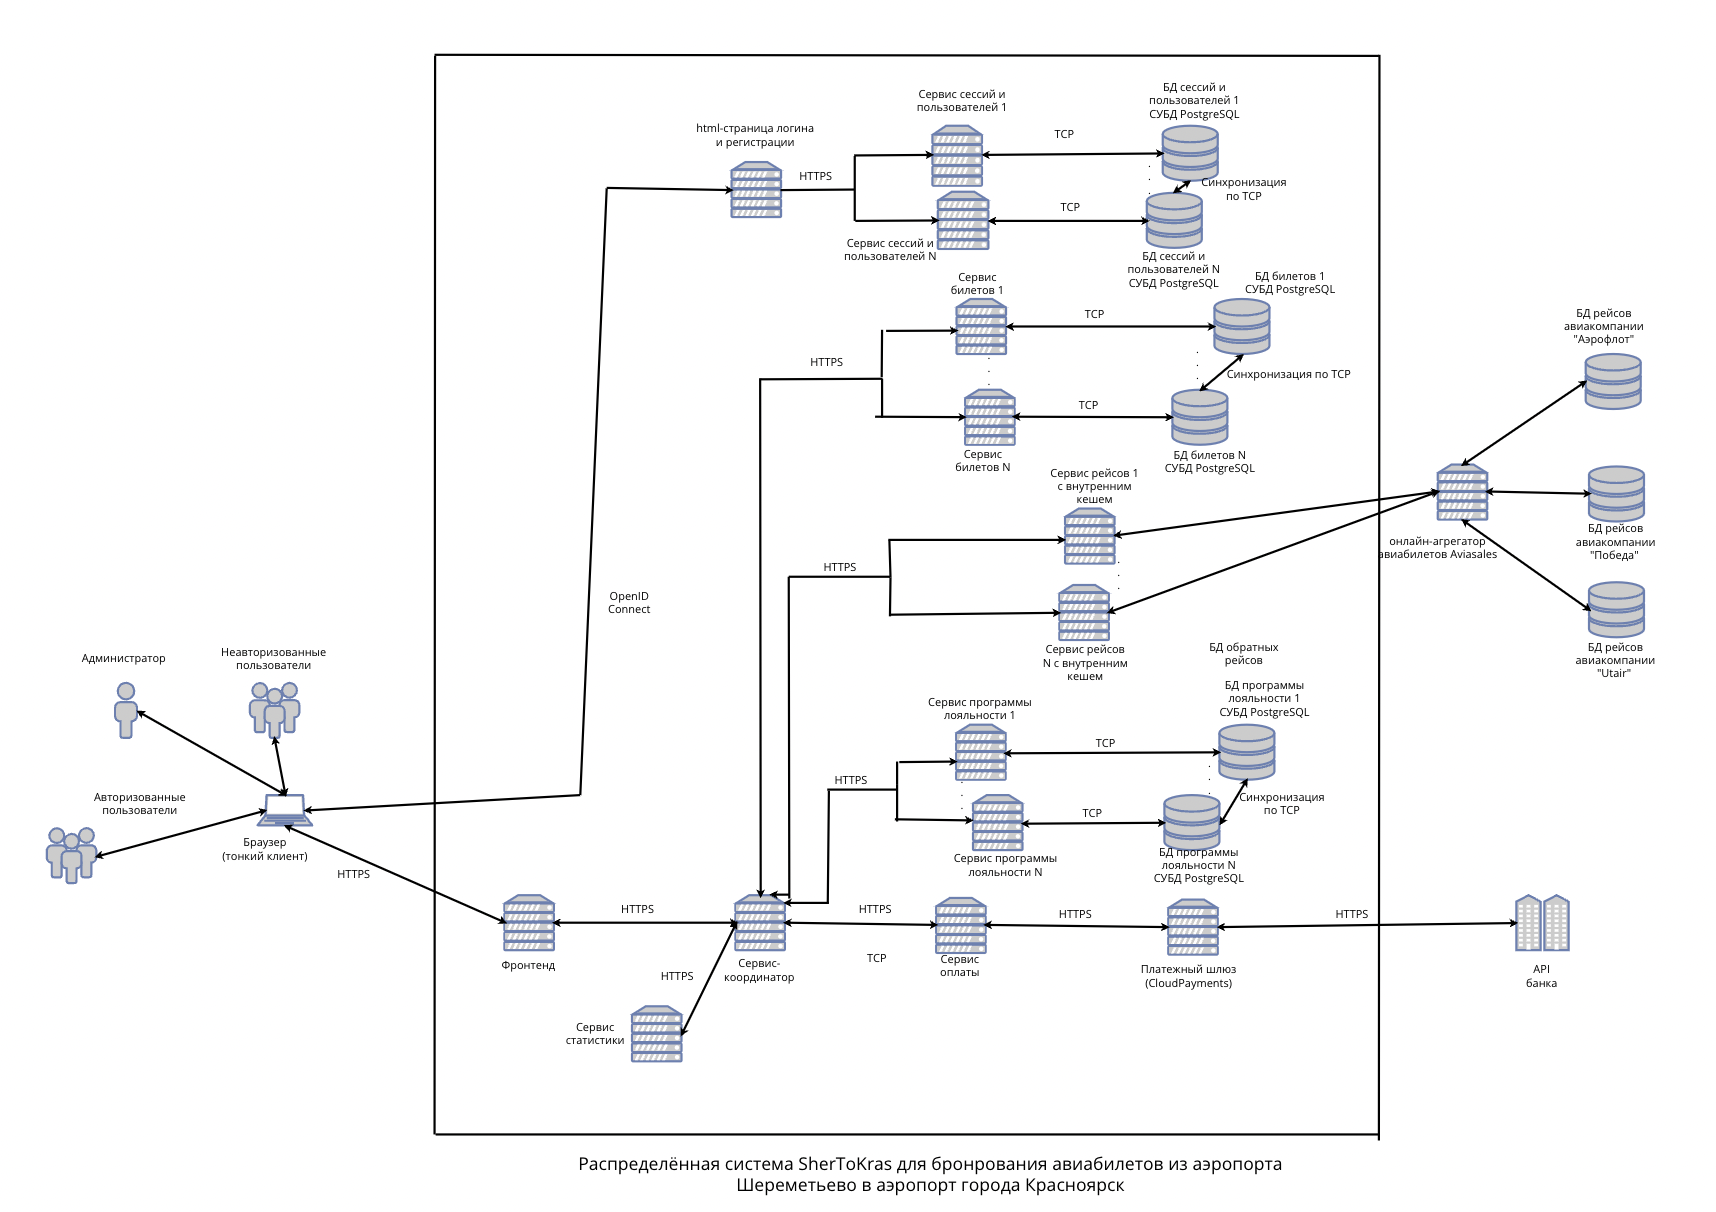
\includegraphics[width=1.05\textwidth]{../images/topology.png}
    \caption{Топология системы}
    \label{images:algorithm}
\end{figure}

\vspace{2em}

Система должна состоять из 2 подсистем:

\begin{itemize}
    \item подсистема авторизации;
    \item подсистема бронирования рейсов.
\end{itemize}

Подсистема бронирования рейсов должна состоять из фронтенда и шести сервисов, что наиболее целесообразно для реализации ее основного назначения. 

Подсистема авторизации должна состоять из одного сервиса и html-страницы с полями для ввода логина и пароля, а также регистрации. 

Взаимодействие подсистемы бронирования авиарейсов с подсистемой авторизации должно осуществляться по протоколу OpenID Connect.

Все сервисы подсистемы бронирования рейсов должны взаимодействовать друг с другом через сервис-координатор, запросы с фронтенда в том числе сначала должны приходить на сервис-координатор, а затем перенаправляться на нужный сервис. 

Сервисы, используемые пользователями часто (сервис сессий и пользователей, сервис-координатор, сервис рейсов, сервис билетов, сервис программы лояльности) должны работать в нескольких экземплярах в разных географических позициях для обеспечения одинаковой задержки при загрузке страниц из разных географических позиций и, соответственно, меньшей нагрузки на сеть.

В рамках данной системы такие узлы размещения определяются на основе вероятных источников пользовательских запросов — это, прежде всего, Москва (аэропорт Шереметьево) и город Красноярск, в которых расположены аэропорты и в которые планируется выполнять авиаперелёты. Такой подход позволяет обеспечить более высокую производительность, устойчивость к сетевым сбоям и более комфортный пользовательский опыт.

В рамках одной географической позиции также могут быть использованы несколько работающих экземпляров сервиса. Нагрузка между сервисами может быть распределена с помощью алгоритма RoundRobin.

При этом некоторые из дублируемых сервисов обращаются к своей локальной копии базы данных, поэтому обязательной становится задача синхронизации данных между этими копиями. Синхронизация осуществляется по протоколу TCP с использованием встроенных механизмов репликации, поддерживаемых большинством популярных СУБД. Такие механизмы позволяют обеспечить согласованность данных между географически распределёнными инстансами баз, сохраняя актуальность информации во всех точках доступа.

Фронтенд должен принимать запросы от пользователя по протоколу HTTP и возвращать ответ в виде HTML страниц, файлов стилей и java script.

Перечислим сервисы и их ответственность в системе.
\begin{enumerate}
    \item Сервис-координатор отвечает за координацию запросов внутри системы. Для реализации балансировки запросов используется инфраструктура Kubernetes.
    \item Сервис сессий и пользователей отвечает за сессию пользователей портала и реализует следующие функции:
    \begin{itemize}
        \item регистрация пользователя (покупателя); 
        \item авторизация пользователя (вход, или <<логин>>);
        \item выход из сессии (<<логаут>>).
        \item получение информации, изменение, удаление покупателя.
    \end{itemize}
    
    Сервис использует в своей работе базу данных. О каждом покупателе хранится следующая информация:
    \begin{itemize}
        \item логин (уникальное в рамках системы текстовое поле, максимум 256 символов);
        \item пароль (текстовое поле, не более 128 символов);
        \item имя и фамилия (каждое является текстовым полем, максимум 256 символов);
        \item Роль (пользователь / администратор);
        \item дата рождения.
    \end{itemize}
    \item Сервис программы лояльности реализует следующие функции:
    \begin{itemize}
        \item узнать баланс на счёте лояльности пользователя и историю изменения счёта лояльности с указанием для каждого события истории: суммы изменения, даты изменения, типа изменения и идентификатора билета, связанного с изменением; 
        \item произвести начисление бонусных баллов при покупке билета; 
        \item произвести списание бонусных баллов при возврате билета (при этом остаток бонусного счёта не может быть меньше 0).
    \end{itemize}

    Сервис программы лояльности использует в своей работе базу данных для хранения текущего баланса и истории изменений бонусного счёта каждого покупателя.

    \item Сервис билетов реализует следующие функции:
    \begin{itemize}
        \item получить информацию о всех купленных билетах пользователя; 
        \item получить информацию о билете пользователя с заданным идентификатором; 
        \item отметить билет купленным или возвращённым.
    \end{itemize}

     Сервис билетов использует в своей работе базу данных. О каждом билете хранится следующая информация:
    \begin{itemize}
        \item уникальный а рамках системы идентификатор билета;
        \item логин пользователя, купившего билет;
        \item идентифкатор рейса;
        \item цена билета;
        \item статус билета (оплачен / возвращён).
    \end{itemize}
    
    \item Сервис рейсов реализует следующие функции:
    \begin{itemize}
        \item получить информацию о всех рейсах; 
        \item получить информацию о рейсе с заданным идентификатором.
    \end{itemize}

    Сервис рейсов не использует собственную базу данных для хранения информации о рейсах. 
    При каждом пользовательском запросе сервис отправляет запрос к API онлайн-агрегатора Aviasales, который предоставляет актуальные данные о рейсах, тарифах и остатках мест. 
    Для повышения производительности и снижения нагрузки на внешний API результаты таких запросов кешируются с использованием Redis.

    При поступлении запроса формируется уникальный ключ кэша, включающий параметры маршрута (например, Шереметьево → Красноярск), дату вылета, количество пассажиров, класс обслуживания и другие необходимые детали. 
    Если по этому ключу в Redis уже есть актуальный кешированный ответ, сервис немедленно возвращает данные из кэша. 
    Если кеш отсутствует или истёк (TTL истёк), происходит обращение к API Aviasales, полученный результат сохраняется в Redis с заранее заданным временем жизни (TTL), и затем отправляется пользователю.

    Выбор времени жизни кеша зависит от специфики авиаданных. 
    В нашем сценарии устанавливается TTL кеша равный 15 минутам. 
    Это означает, что результаты запроса к Aviasales будут сохраняться в Redis в течение 15 минут, что позволяет существенно снизить нагрузку на внешний API при повторных запросах от пользователей. 
    При этом, поскольку динамические данные (например, цены, наличие мест или актуальный статус рейса) могут изменяться даже в пределах этого интервала, в процессе оформления билета проводится финальная проверка: перед бронированием сервис всегда обращается к API Aviasales для уточнения и обновления динамических параметров. 
    Таким образом, даже если пользователь изначально получил результаты из кеша, актуальность данных гарантируется за счёт дополнительного запроса при покупке, что обеспечивает баланс между быстродействием (благодаря Redis-кешированию) и точностью предоставляемой информации.

    О каждом рейсе хранится следующая информация:
    \begin{itemize}
        \item уникальный а рамках системы идентификатор рейса;
        \item дата полёта;
        \item аэропорт отправления;
        \item аэропорт назначения;
        \item цена рейса.
    \end{itemize}

    \item Сервис оплаты отвечает за проведение операций по оплате и возврату билетов через внешний платёжный шлюз CloudPayments. Он получает запрос от координатора, регистрирует платёж и перенаправляет его в шлюз. После обработки транзакции CloudPayments сообщает результат, который фиксируется в системе и используется для завершения бронирования или возврата. Сервис обеспечивает надёжную и безопасную оплату с последующим уведомлением всех необходимых компонентов системы.
    
    \item Сервис статистики отвечает за логирование событий во всей системе для осуществления возможности быстрого детектирования, локализации и воспроизведения ошибки в случае её возникновения. 
\end{enumerate}

\section*{Требования по реализации со стороны заказчика}
\addcontentsline{toc}{section}{Требования по реализации со стороны заказчика}

\begin{enumerate}
	\item Требуется использовать сервис-ориентированную архитектуру для реализации системы.
    \item Требуется использование очереди сообщений Kafka для повышения отказоустойчивости системы.
	\item Система состоит из микросервисов. Каждый микросервис отвечает за свою область логики работы приложения.
	\item Взаимодействие между сервисами осуществляется посредством HTTP запросов.
	\item Данные сервисов должны храниться в базе данных. Каждый сервис взаимодействует только со своей схемой данных. Взаимодействие сервисов происходит по технологии REST.
	\item При недоступности систем портала должна осуществляться деградация функциональности или выдача пользователю сообщения об ошибке.
	\item Необходимо предусмотреть авторизацию пользователей через интерфейс приложения.
	\item Для авторизации использовать протокол OpenID Connect.
	\item Для запросов, выполняющих обновление данных на нескольких узлах распределенной системы, в случае недоступности одной из систем, необходимо выполнять полный откат транзакции.
	\item Приложение должно поддерживать возможность горизонтального и вертикального масштабирования за счет увеличения количества функционирующих узлов и совершенствования технологий реализации компонентов и всей архитектуры системы.
\end{enumerate}


\section*{Функциональные требования по подсистемам}
\addcontentsline{toc}{section}{Функциональные требования по подсистемам}

\begin{enumerate}
    \item Фронтенд -- это серверное приложение при разработке которого необходимо учитывать следующие факторы:
    \begin{itemize}
        \item фронтенд должен принимать запросы по протоколу HTTPS и формировать ответы пользователям портала в формате HTML;
        \item в зависимости от типа запроса фронтенд должен отправлять последовательные запросы в соответствующие бекенды;
        \item запросы к бекендам необходимо осуществляет по протоколу HTTPS; данные необходимо передавать в формате JSON;
        \item требуется использование веб-сервиса Nginx для более быстрого возврата пользователям статического содержимого (изображения, таблиц стилей, JavaScript файлов), а также для балансировки запросов к нескольким экземплярам сервиса-координатора.
    \end{itemize}
    \item Сервис пользователей, сервис сессий, сервис программы лояльности, сервис рейсов и сервис билетов -- это серверные приложения, которые должны отвечать следующим требованиям по разработке:
    \begin{itemize}
        \item обрабатывать запросы в соответствии со своим назначением, описанным в топологии системы;
        \item принимать и возвращать данные в формате JSON по протоколу HTTPS;
        \item осуществлять доступ к СУБД по протоколу TCP.
    \end{itemize}
    \item Сервис-координатор -- это серверное приложение, которое должно отвечать следующим требованиям по разработке:
    \begin{itemize}
        \item обрабатывать запросы в соответствии со своим назначением, описанным в топологии системы;
        \item принимать и возвращать данные в формате JSON по протоколу HTTPS;
        \item использовать очередь для отложенной обработки запросов (например, при временном отказе одного из сервисов);
        \item осуществлять деградацию функциональности в случае отказа некритического сервиса (зависит от семантики запроса);
        \item существовать в нескольких экземплярах, чтобы координация запросов не была узким местом приложения;
        \item уведомлять сервис статистики о событиях в системем.
    \end{itemize}
    \item Сервис статистики и сервис оплаты -- это серверные приложения, которые должны отвечать следующим требованиям по разработке:
    \begin{itemize}
        \item обрабатывать запросы в соответствии со своим назначением, описанным в топологии системы;
        \item принимать и возвращать данные в формате JSON по протоколу HTTPS.
    \end{itemize}
\end{enumerate}

\section*{Сценарий взаимодействия фронтенда и бекендов}
\addcontentsline{toc}{section}{Сценарий взаимодействия фронтенда и бекендов}

Рассмотрим, как взаимодействуют фронтенд и бекенды на примере выполнения запроса от пользователя на получение списка рейсов.

\begin{enumerate}
    \item На фронтенд приходит данный запрос пользователя.
    \item Фронтенд анализирует запрос пользователя и, если пользователь был авторизован ранее, получает из него JWT-токен. Далее выполняется запрос к сервису-координатору. Координатор проверяет корректность полученных данных (того, что данные поступили в ожидаемом формате, то есть в формате, соответствующем протоколу взаимодействия). Координатор отправляет запрос на сервис рейсов. В сервисе рейсов осуществляется проверка корректности полученных данных (того, что данные поступили в ожидаемом формате, то есть в формате, соответствующем протоколу взаимодействия) и проверка JWT-токен-а (проверка того, что токен был подписан известным серверу ключом и того, что срок действия токена ещё не истёк). Если он истёк или оказался некорректным, пользователю возвращается ошибка. При успешной проверке токена сервис возвращает список рейсов сервису-координатору, который в свою очередь возвращает результат на фронтенд.
    \item Если ошибки нигде не произошло, то производится генерация HTML содержимого страницы ответа пользователю с использованием данных, полученных от сервиса рейсов. В ином случае генерируется страница с описанием ошибки.
\end{enumerate}

\section*{Сценарий взаимодействия бекендов}
\addcontentsline{toc}{section}{Сценарий взаимодействия бекендов}

Сервис‑координатор — это серверное приложение, отвечающее следующим требованиям по разработке. 
Оно использует уже существующие решения, такие как Apache Kafka, которая необходима для сбора и обработки данных в реальном времени, что позволяет анализировать пользовательскую активность. 
Kafka способна обрабатывать высокие объёмы данных и легко масштабируется, обеспечивая надёжную работу даже при значительных нагрузках. 
При этом сама Kafka может быть развернута в Kubernetes с использованием Helm‑чартов или Strimzi Kafka Operator, что позволяет автоматически управлять жизненным циклом брокеров, настройками сети, хранением данных через StatefulSet и PersistentVolumeClaims, а также обновлениями и масштабированием.

Для управления Kafka из программного кода мы используем библиотеку на языке Python confluent\_kafka.

Чтобы сервис‑координатор получал внешние запросы, обычно настраивается Kubernetes Ingress, который позволяет описывать правила маршрутизации (на основе URL или доменного имени) и направлять HTTP‑запросы от пользователей непосредственно к сервису‑координатору. 
Таким образом, Kubernetes Ingress в сочетании с развернутой в Kubernetes Kafka обеспечивает полную инфраструктуру для высоконагруженной и надёжной обработки запросов: Ingress отвечает за внешние подключения, а Kafka – за асинхронную очередь сообщений, которая организует последовательную обработку поступающих задач даже при пиковых нагрузках.

Теперь рассмотрим сценарии взаимодействия бекендов при различных запросах пользователя:

\begin{enumerate}

    \item Поиск рейсов пользователем
    \begin{itemize}
        \item \textbf{Поступление запросов (Kubernetes Ingress → Сервис‑координатор)}
        \begin{enumerate}
            \item Пользователь на фронтенде выбирает фильтры по которым будет делать запрос на просмотр рейсов и нажимает кнопку "Найти рейсы"
            \item Запрос отправляется в кластер Kubernetes и проходит через Kubernetes Ingress, где согласно настройкам маршрутизации (host/URL‑правила) перенаправляется непосредственно на Сервис‑координатор.
        \end{enumerate}
        \item \textbf{Публикация сообщения в очередь Kafka}

        Сервис‑координатор публикует сообщение в соответствующий топик Kafka (flights\_search\_requests).
        \item \textbf{Проверка доступности и получение данных (Сервис рейсов с Redis и прямым API)}

        Сервис рейсов подписан на этот топик и, получив сообщение, проверяет свой кэш (TTL 15 минут):
        \begin{itemize}
            \item Если подходящие данные есть в Redis кэше, сервис рейсов сразу возвращает их.
            \item Если в кеше ничего нет, то мы обращаемся через API Aviasales напрямую за информацией по этому рейсу.
            \item Перед отправкой запроса в API Aviasales, данные, полученные от пользователя, необходимо предварительно преобразовать в новый формат, соответствующий требованиям и спецификациям Aviasales.
        \end{itemize}

        \item \textbf{Обработка результата запроса}
        \begin{itemize}
            \item По завершении (независимо от успеха или ошибки) сервис рейсов формирует событие (FlightSearchResult), в котором указывает итоговый статус и данные (либо ошибку).
            \item Публикация события в отдельный топик «flights\_search\_responses».
            \item Сервис статистики подписан на этот топик, поэтому информации о результате запроса записывается в журнал.
        \end{itemize}

        \item \textbf{Возврат данных на фронтенд}
        \begin{itemize}
            \item Фронтенд получает JSON-ответ, в котором содержится подробная информация по каждому найденному рейсу. 
            \item На основе этой структуры JSON клиентская часть формирует динамический контент: пользователь видит список доступных перелётов, их стоимость, время вылета и прочие детали, отфильтрованные согласно исходным параметрам.
        \end{itemize}

    \end{itemize}

    \item Бронирование рейса пользователем
    \begin{itemize}

        \item \textbf{Поступление запросов (Kubernetes Ingress → Сервис‑координатор)}
        \begin{itemize}
            \item Пользователь на фронтенде выбирает рейс (маршрут, дату, класс обслуживания, количество пассажиров) и нажимает кнопку «Забронировать».
            \item Запрос отправляется в кластер Kubernetes и проходит через Kubernetes Ingress, где согласно настройкам маршрутизации (host/URL‑правила) перенаправляется непосредственно на Сервис‑координатор.
        \end{itemize}

        \item \textbf{Публикация сообщения в очередь Kafka}
        Сервис‑координатор публикует сообщение в соответствующий топик Kafka (flight\_detail\_requests).

        \item \textbf{Получение данных о рейсе}
        \begin{itemize}
            \item Сервис рейсов подписан на этот топик и получив сообщение игнорируя кеш обращается к API Aviasales за детальной информацией о рейсе.
            \item Перед отправкой запроса в API Aviasales, данные, полученные от пользователя, необходимо предварительно преобразовать в новый формат, соответствующий требованиям и спецификациям Aviasales.
        \end{itemize}
        
        \item \textbf{Публикация события бронирования (Kafka)}
        \begin{itemize}
            \item Если проверка подтверждает, что билет всё ещё доступен и данные актуальны, cервис-координатор формирует событие BookingRequestCreated с подробностями бронирования (маршрут, цена, данные пассажиров, ID запроса) и публикует его в топик Kafka (например, bookingRequests).
            \item Это событие автоматически доступно для всех сервисов, подписанных на этот топик.
        \end{itemize}

        \item \textbf{Обработка оплаты (Payment Service)}
        \begin{itemize}
            \item Сервис оплаты слушает событие BookingRequestCreated (в топике booking\_requests).
            \item Инициирует транзакцию через платёжный шлюз (CloudPayments, банк и т.п.).
            \item Публикует результат:
            \begin{enumerate}
                \item При успехе: событие PaymentApproved в топик payment\_approved.
                \item При неудаче: событие PaymentFailed в топик payment\_failed.
            \end{enumerate}
            \item Если на шаге финального обновления в Aviasales возникнет ошибка (описано в пункте об «Уведомлении Aviasales и финальном бронировании»), потребуется инициировать refund (возврат средств). В таком случае сервис оплаты будет слушать событие наподобие AviasalesUpdateFailed и проводить возврат (если политика возвратов это допускает), публикуя PaymentRefundSucceeded или PaymentRefundFailed.
        \end{itemize}

        \item \textbf{Уведомление Aviasales и финальное бронирование}
        \begin{itemize}
            \item После получения события PaymentApproved Сервис рейсов (или Сервис-координатор) запрашивает API Aviasales, уведомляя, что билет куплен и данные должны обновиться.
            \item При успешном обновлении Aviasales сервис публикует событие AviasalesUpdateSuccess в топик aviasales\_update\_success:
            \begin{enumerate}
                \item Сервис билетов подписан на aviasales\_update\_success, получает подтверждение и формирует финальную бронь (PNR, e‑ticket).
                \item Публикует событие ReservationConfirmed (в топик reservation\_confirmed), сигнализируя, что бронирование завершено.
                \item Пользователь получает уведомление от Сервиса уведомлений (слушающего reservation\_confirmed).
            \end{enumerate}
            \item Если Aviasales возвращает ошибку (не удалось обновить информацию):
            \begin{enumerate}
                \item Сервис рейсов/координатор публикует событие AviasalesUpdateFailed в топик aviasales\_update\_failed.
                \item Сервис оплаты или координатор, подписанный на aviasales\_update\_failed, инициирует возврат средств (refund) путём публикации команды PaymentRefundRequested.
                \item В случае успеха возврата публикуется PaymentRefundSucceeded, при сбое — PaymentRefundFailed.
                \item Сервис уведомлений информирует пользователя о том, что бронирование не состоялось и платёж возвращён (или не возвращён при PaymentRefundFailed), а Сервис статистики фиксирует негативный сценарий.
            \end{enumerate}
        \end{itemize}

        \item \textbf{Пост-обработка}
        \begin{itemize}
            \item Сервис лояльности также получает событие ReservationConfirmed (или отдельное событие PointsAwarded, инициированное после бронирования) для начисления бонусных миль/баллов пользователю.
            \item Сервис статистики подписан на ВСЕ ключевые топики (например, booking\_requests, payment\_approved, payment\_failed, reservation\_confirmed, aviasales\_updates):
            \begin{enumerate}
                \item Он собирает информацию о количестве успешных и неудачных бронирований, времени отклика на каждое событие, динамике цен и других метриках.
                \item Такая сборка статистики обеспечивает аналитическую базу для оптимизации процессов и оценки качества сервиса.
            \end{enumerate}
        \end{itemize}

    \end{itemize}

    \item Просмотр пользователем личного кабинета
    \begin{itemize}
        \item \textbf{Поступление запросов (Kubernetes Ingress → Сервис‑координатор)}
        \begin{itemize}
            \item Пользователь заходит на страницу личного кабинета.
            \item Запрос отправляется в кластер Kubernetes и проходит через Kubernetes Ingress, где согласно настройкам маршрутизации (host/URL‑правила) перенаправляется непосредственно на Сервис‑координатор.
        \end{itemize}

        \item \textbf{Публикация сообщения в очередь Kafka}
        Сервис‑координатор формирует событие, содержащее детали запроса, и публикует его в топик Kafka, например, \texttt{personal\_cabinet\_requests}.

        \item \textbf{Взаимодействие с сервисом авторизации}
        \begin{itemize}
            \item Сервис авторизации, подписанный на соответствующий топик или получающий запрос от Сервис‑координатора, проверяет наличие данных пользователя.
            \item Если данные пользователя найдены:
            \begin{itemize}
                \item Сервис авторизации публикует событие (например, \texttt{UserDataFound}) с информацией о пользователе в топик, на который подписан Сервис‑координатор.
                \item Сервис‑координатор получает событие, отправляет данные о пользователе на фронтенд, обеспечивая показ личного кабинета.
            \end{itemize}
            \item Если данных пользователя не найдено:
            \begin{itemize}
                \item Сервис авторизации инициирует перенаправление (или публикует соответствующее событие, например, \texttt{UserDataMissing}), что приводит к переходу пользователя на страницу регистрации.
            \end{itemize}
        \end{itemize}

        \item \textbf{Публикация данных в сервис статистики}
        \begin{itemize}
            \item Независимо от результата (успех или отсутствие данных), событие о результате запроса публикуется в топик для статистики, например, \texttt{personal\_cabinet\_responses}, который подписан на этот.
        \end{itemize}

        \item \textbf{Возврат данных на фронтенд}
        \begin{itemize}
            \item Сервис‑координатор, подписанный на \texttt{personal\_cabinet\_responses}, получает событие об итоговом статусе:
                \begin{itemize}
                    \item Если это \texttt{UserDataFound}, координатор передаёт на фронтенд JSON-объект с данными пользователя (имя, фамилия, e-mail и т.п.).
                    \item Если это \texttt{UserDataMissing}, координатор перенаправляет пользователя (или возвращает ответ фронтенду), указывая, что необходимо перейти на страницу регистрации.
                \end{itemize}
        \end{itemize}

    \end{itemize}

    \item Просмотр пользователем забронированных им рейсов
    \begin{itemize}
        \item \textbf{Поступление запросов (Kubernetes Ingress → Сервис‑координатор)}
        \begin{itemize}
            \item Пользователь находясь на странице личного кабинета, нажимает на пункт меню "Мои бронирования".
            \item Запрос включает JWT-токен, который передаётся через Ingress в Сервис‑координатор.
        \end{itemize}

        \item \textbf{Получение user\_id через Сервис авторизации}
        \begin{itemize}
            \item Сервис‑координатор извлекает JWT-токен и отправляет его в Сервис авторизации.
            \item Сервис авторизации проверяет токен и возвращает уникальный идентификатор пользователя (user\_id).
        \end{itemize}

        \item \textbf{Публикация запроса в очередь Kafka}
        \begin{itemize}
            \item Сервис‑координатор формирует сообщение запроса, включающее user\_id и другие необходимые параметры.
            \item Сообщение публикуется в топик Kafka, например, \texttt{user\_bookings\_requests}.
        \end{itemize}

        \item \textbf{Обработка запроса (Сервис билетов)}
        \begin{itemize}
            \item Сервис билетов, подписанный на \texttt{user\_bookings\_requests}, получает сообщение.
            \item Используя user\_id, сервис билетов осуществляет поиск бронирований в своей базе данных.
            \item Результат (список бронирований) формируется и публикуется в топик \texttt{user\_bookings\_responses}.
        \end{itemize}

        \item \textbf{Отправка данных в Сервис статистики}

        Сервис статистики подписан на топик \texttt{user\_bookings\_responses}, и при публикации сообщения в этот топик, информация передается в сервис статистики для журналирования.

        \item \textbf{Возврат данных на фронтенд}
        \begin{itemize}
            \item Фронтенд получает JSON-ответ с массивом забронированных рейсов:
            \begin{itemize}
                \item Если массив пустой, пользователю отображается сообщение «Нет активных бронирований».
                \item Если в JSON содержатся данные, пользователь видит список своих текущих рейсов с ключевой информацией (номер рейса, время вылета и т.д.).
            \end{itemize}
        \end{itemize}

    \end{itemize}

\end{enumerate}

\section*{Пользовательский интерфейс}
\addcontentsline{toc}{section}{Пользовательский интерфейс}

Для реализации пользовательского интерфейса должен быть использован подход MVC (Model-View-Controller). Этот подход к проектированию интерфейса является популярным шаблоном проектирования, который помогает разделить логику приложения на три основных компонента: Модель (Model), Представление (View) и Контроллер (Controller). Этот подход позволяет улучшить структуру приложения, облегчить его тестирование и управление, а также разработка фронтенда и бекенда могут быть полностью разделены между собой, то есть можно вести независимую разработку.

Пользовательский интерфейс в разрабатываемой системе должен обладать следующими характеристиками:
\begin{itemize}
    \item Адаптивность к размеру экрана устройства пользователя -- пользовательский интерфейс <<подстраивается>> под всевозможные размеры экранов устройств: мобильных телефонов, планшетов, ноутбуков и т.д.
    \item Кроссбраузерность -- способность интерфейса работать практически в любом браузере любой версии. 
    \item <<Плоский» дизайн>>>> -- дизайн, в основе которого лежит идея отказа от объемных элементов (теней элементов, объемных кнопок и т.д.) и замены их плоскими аналогами.
    Данная технология становится популярной в последнее время по ряду причин:
    \begin{enumerate}
        \item Простота поддержки.
        \item Упор на развитую функциональность, а не на красоту интерфейса.
        \item Сокращение затрат на разработку дизайна.
    \end{enumerate}
    \item Расширяемость -- возможность легко расширять и модифицировать пользовательский интерфейс. 
    Интерфейс спроектирован таким образом, чтобы его можно было дополнять новыми компонентами, не нарушая текущую структуру и логику взаимодействия.
    Модульность вёрстки и кода: каждая функциональная часть (виджет, панель, меню) оформлена как самостоятельный блок (компонент), который можно добавлять, удалять или заменять без полной перестройки всего интерфейса.
    \item Интуитивно понятный интерфейс -- все кнопки имеют подписи при наведении на них, многие содержат иконки, облегчающие восприятие пользователем.
\end{itemize}

Пользовательский интерфейс в разрабатываемой системе представляет собой web-интерфейс, доступ к которому осуществляется через браузер (тонкий клиент). Страница системы состоит из «шапки», основной части.

Обобщенно структуру страниц системы можно представить следующим образом:

\begin{itemize}
    \item главная страница с поиском авиабилетов;
    \item страница подробной информацией о билете и кнопкой покупки;
    \item личный кабинет пользователя (информация о пользователе с возможно- стью ее изменить);
    \item страница с купленными билетами (с возможностью вернуть еще не использованные билеты);
    \item страница программы лояльности (история операций бонусного счета, остаток на бонусном счёте);
    \item страница входа;
    \item страница регистрации;
    \item страница со статистикой запросов в приложении (доступно администраторам);
\end{itemize}

\section*{Требования к дизайну}
\addcontentsline{toc}{section}{Требования к дизайну}

Дизайн веб-сайта системы бронирования авиабилетов должен быть минималистичным, удобным и интуитивно понятным.
В оформлении системы бронирования предполагается использовать сине-белую цветовую гамму — такой выбор символизирует небо и облака, тесно связанные с авиаперелётами. 
Сочетание синего фона и белых элементов подчёркивает тематику сайта и формирует лёгкое, «воздушное» восприятие интерфейса, что соответствует идее комфортных авиапутешествий. 
Интерфейс должен быть адаптивным для удобной работы как на компьютерах, так и на мобильных устройствах.

\begin{enumerate}
    \item \textbf{Главная страница бронирования авиабилетов}

        \textbf{Цель страницы:} представить пользователям сервис бронирования авиабилетов, предоставить быстрый доступ к основным функциям (поиск, авторизация)
        \begin {itemize}
            \item \textbf{Шапка (header):}
            \begin{itemize}
                \item Крупный текст «Путешествовать стало проще», который привлекает внимание и подчёркивает идею быстрого/лёгкого бронирования.
            \end{itemize}
            \item \textbf{Основной блок (середина):}
            \begin{itemize}
                \item Выбор города вылета (по умолчанию «Москва (SVO)»).
                \item Поле «Куда летим?» — текстовое поле (placeholder), куда пользователь вводит или выбирает аэропорт назначения.
            \end{itemize}
            \item \textbf{Подвал (footer):}
            \begin{itemize}
                \item Набор иконок внизу экрана (примерно три-четыре пункта):
                \item Значок «Поиск» (активен на текущей странице).
                \item Другие иконки (например, «Билеты», «Профиль», «Дополнительно»), обеспечивающие доступ к другим страницам.
            \end{itemize}
        \end{itemize}

    \item \textbf{Страница авторизации}

        \textbf{Цель страницы:} Предоставить пользователю удобный способ войти в свой профиль для бронирования авиабилетов. Упростить процесс входа за счёт интеграции с социальными сетями (Google, Facebook и т.д.).
        \begin {itemize}
            \item \textbf{Шапка (header):}
            \begin{itemize}
                \item \textbf{Фоновое изображение:} Верхнюю часть экрана занимает яркий сине-белый фон с облаками, на котором изображён самолёт в полёте. Сцена визуально передаёт тему авиапутешествий и задаёт общий «воздушный» стиль приложения.
                \item \textbf{Заголовок "Вход"/"Регистрация":} Размещён по центру, поверх фона с самолётом. Этот заголовок чётко указывает на назначение страницы — авторизацию пользователя.
            \end{itemize}
            \item \textbf{Основной блок (середина):}
            \begin{itemize}
                \item \textbf{Форма авторизации:}
                \begin{enumerate}
                    \item \textbf{Поле «Введите e-mail»:} текстовое поле для ввода электронной почты.
                    \item \textbf{Поле «Введите пароль»:} скрытое поле для пароля.
                    \item \textbf{Кнопка «Login»:} расположена сразу под полями ввода, обычно выделена синим или контрастным цветом для привлечения внимания.
                \end{enumerate}
                \item \textbf{Быстрый вход через соцсети:} Прямо под кнопкой «Login» отображаются иконки (Google, Facebook), которые позволяют авторизоваться, используя учётные записи из популярных социальных сетей.
            \end{itemize}
            \item \textbf{Подвал (footer):}
            \begin{itemize}
                \item \textbf{Ссылка для регистрации:} надпись «Нет аккаунта? Зарегистрироваться», обычно располагается внизу экрана. Пользователь может нажать на «Зарегистрироваться» и перейти к форме создания нового профиля.
            \end{itemize}
        \end{itemize}

    \item \textbf{Страница личного кабинета}

        \textbf{Цель страницы:} Предоставить пользователю централизованное пространство для управления своей учётной записью в сервисе бронирования авиабилетов, где он может просматривать и редактировать личные данные, получать доступ к бронированиям, бонусной программе и дополнительным настройкам, а также обращаться в службу поддержки — обеспечивая тем самым персонализированный и удобный опыт использования сервиса.
        \begin{itemize}
            \item \textbf{Шапка (header)}
            \begin{enumerate}
                \item \textbf{Отображение учётной записи:}
                \begin{itemize}
                    \item В верхней части экрана указаны e-mail пользователя и дополнительная информация (город «Москва, Россия»).
                    \item Значок «>» справа может указывать на переход к детальным настройкам профиля или выпадающему меню.
                \end{itemize}
                \item \textbf{Фоновый стиль:}
                \begin{itemize}
                    \item Шапка выделена цветом или визуальной границей, в целом выдерживая общую сине-белую цветовую гамму, характерную для авиасервиса.
                    \item Здесь же может быть кнопка «назад» или «закрыть», если это боковая панель (меню).
                \end{itemize}
            \end{enumerate}
            \item \textbf{Основной блок (середина)}
                \begin{itemize}
                    \item \textbf{Профиль:} Переход к деталям учётной записи, где можно редактировать личные данные, фотографию и т.д.
                    \item \textbf{Бонусная программа:} Отдельный раздел для накопления миль/баллов и просмотра текущего баланса.
                    \item \textbf{Мои бронирования:} История и статус приобретённых билетов, доступ к посадочным талонам, деталям перелётов.
                    \item \textbf{Данные пассажира:} Ввод или редактирование паспортных данных, предпочтений (бортовое питание, место), которые будут использоваться при следующих бронированиях.
                    \item \textbf{Поддержка:} Ссылка на FAQ, чат или форму отправки запросов в службу поддержки.
                    \item \textbf{Контакты:} Адреса, телефоны и e-mail, по которым можно связаться со службой сервиса.
                    \item \textbf{Настройки:} Дополнительные параметры приложения: язык интерфейса, уведомления, персональные предпочтения.
                \end{itemize}
            \item \textbf{Подвал (footer)}
                \begin{itemize}
                    \item Логотип компании или краткое упоминание сервиса в самом низу.
                    \item Версию приложения или года действия лицензии.
                    \item Кнопку выхода (лог-аут), если она не размещена в основном списке.
                \end{itemize}
        \end{itemize}

    \item \textbf{Страница мои бронирования}
        
        \textbf{Цель страницы:} Позволить пользователю быстро просмотреть все ранее оформленные (или предстоящие) авиабилеты, узнать детали по каждому рейсу (аэропорт, дату/время вылета и прилёта, авиакомпанию, класс обслуживания), а при необходимости перейти к дополнительной информации или управлению бронированием.
        \begin{itemize}
            \item \textbf{Шапка (header)}
                \begin{enumerate}
                    \item \textbf{Заголовок «Мои бронирования»} Крупным шрифтом в верхней части экрана указано название страницы, чтобы пользователь понимал, что это список всех его приобретённых перелётов.
                    \item \textbf{Кнопка назад или меню} В левом верхнем углу может располагаться стандартная «стрелка» для возврата на предыдущий экран (или иконка меню, если дизайн приложения предполагает боковую навигацию).
                \end{enumerate}
            \item \textbf{Основной блок (середина)}
                \begin{enumerate}
                    \item \textbf{Список (карточки) забронированных рейсов} : каждая карточка влючает в себе следующую информацию:
                    \begin{itemize}
                        \item Маршрут (указывающий аэропорт вылета/прилёта)
                        \item Дата и время вылета
                        \item Дата и время прилета 
                        \item Информация об авиакомпании
                    \end{itemize}
                    \item \textbf{Множественные записи:} Если у пользователя несколько бронирований, они идут списком (карточками), каждое содержит уникальные данные: даты, время, авиакомпанию, маршрут.
                    \item \textbf{Кликабельность:} Каждая карточка может вести на детальную страницу бронирования (при нажатии), где пользователь увидит посадочные талоны, правила возврата, дополнительные опции (покупка багажа, выбор места и т.п.).
                \end{enumerate}
            \item \textbf{Подвал (footer)}
            \begin{itemize}
                \item \textbf{Навигационные элементы}
                \begin{enumerate}
                    \item Приложение имеет стандартную нижнюю панель навигации (с иконками «Главная», «Поиск», «Мои бронирования», «Профиль» и т.д.).
                    \item Текущая вкладка («Мои бронирования») может быть подсвечена, чтобы пользователь знал, что находится на странице бронирований.
                \end{enumerate}
            \end{itemize}
        \end{itemize}    

\end{enumerate}

\section*{Требования к составу и параметрам технических средств}
\addcontentsline{toc}{section}{Требования к составу и параметрам технических средств}

Все серверные приложения должны потреблять суммарно не более 2 Гбайт оперативной памяти и работать на сервере с процессором Intel(R) Core(TM) i7- 10510U CPU 1.80GHz.

\section*{Требования к надежности}
\addcontentsline{toc}{section}{Требования к надежности}

Система должна работать в соответствии с данным техническим заданием без перезапуска.
Необходимо использовать <<зеркалируемые серверы>> для всех подсистем, которые будут держать нагрузку в случае сбоя до тех пор, пока основной сервер не восстановится.

\section*{Требования к документации}
\addcontentsline{toc}{section}{Требования к документации}

Исполнитель должен подготовить и передать Заказчику следующие документы:

\begin{itemize}
    \item руководство по развертыванию Системы;
    \item руководство администратора Системы;
    \item руководство для покупателя по использованию Системы.
\end{itemize}